\chapter{安全分析の基本手法: FTAとFMEA}
\label{chap2}
\section{未然防止の手法}
障害への対応法は、応急処置、再発防止、および未然防止がある。応急処置、再発防止は発生した障害に対応する事後解析であり、リアクティブな方法(Reactive Approach)と呼ばれる。未然防止は、障害が発生してから対策を取るのではなく、計画段階や設計段階の生産の源流において、将来起こりうる障害を洗い出して、それらに対策を講じてしまうことである。潜在的な障害に対応する事前解析であり、プロアクティブな方法(proactive approach)といわれる。未然防止の手法には、FMEA(Failure Mode and Effect Analysis), FTA(Fault Tree Analysis), ETA(Event Tree Analysis), 良品解析などがある。信頼性工学や安全性工学では良さ加減を増強するよりも、悪さ加減を減少させる方法がとられることが多い。

未然防止技術は多くある(多変量解析、品質機能展開、品質工学、実験計画法、WCA、FEM、信頼性試験、故障解析、信頼性データ解析、リスク・アセスメント、ライフサイクル・アセスメント(LCA))。本講義では、最も代表的なFTA, FMEAを扱う。
\section{FTAとFMEA}
 FMEA, FTAは対象とするシステム(製品、設備、プロセスなど)の故障、不具合、欠陥などの「悪さ加減」を論理的に洗い出して、内在する問題点を発見する解析手法である。見出された問題点に対しては、実際の技術活動や管理活動を通じて対策や是正措置が取られる。
 
FTAとFMEAの形態を示す。図\ref{191}、図\ref{192}は、工作用の洋ばさみについてのFTAとFMEAである。
\begin{figure}[htbp]
\begin{center}
%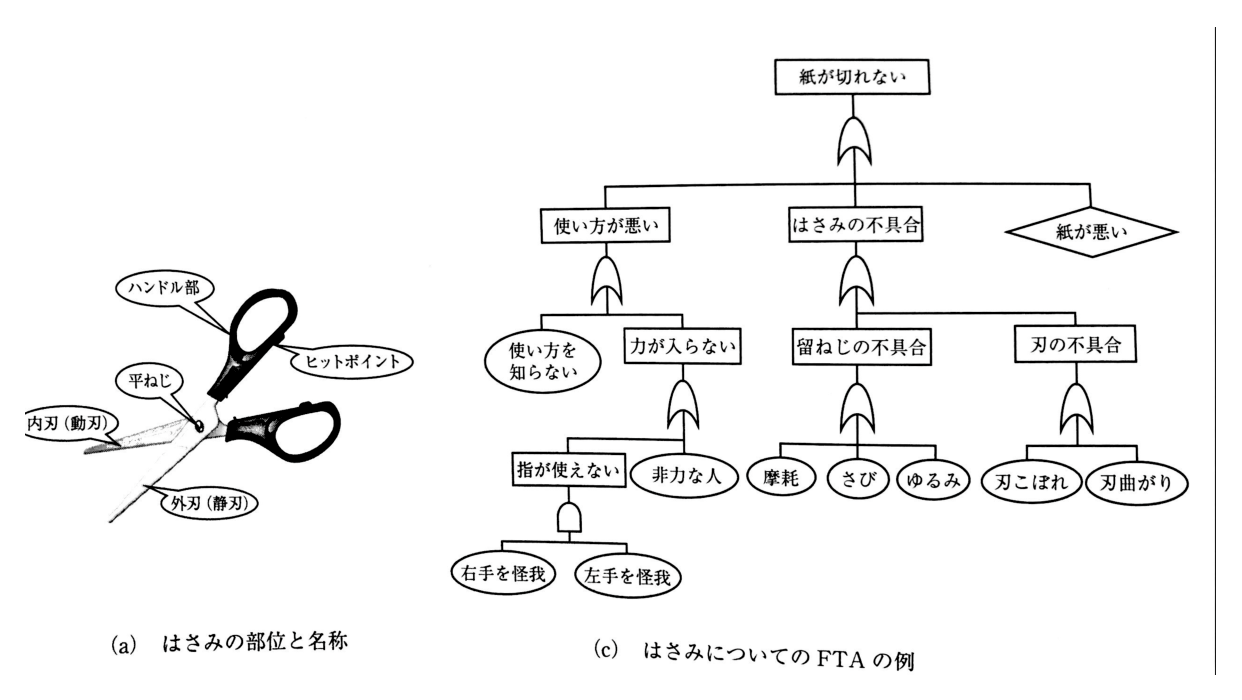
\includegraphics[width=15cm]{safety_assurance_contents/ch2images/191}
\end{center}
\caption{FTAの形態(工作用はさみの事例)}
\label{191}
\end{figure}
(a)ははさみの部分と名称を示したもので、内刃、外刃、留ねじの3つの部品からなる。(b)ははさみに対して実施した設計FMEAを示す。部品の故障モードを洗い出して、システム(この場合ははさみ)への影響を表形式で解析する手法である。原因系から結果系を予測する方法と言える。
\begin{figure}[htbp]
\begin{center}
%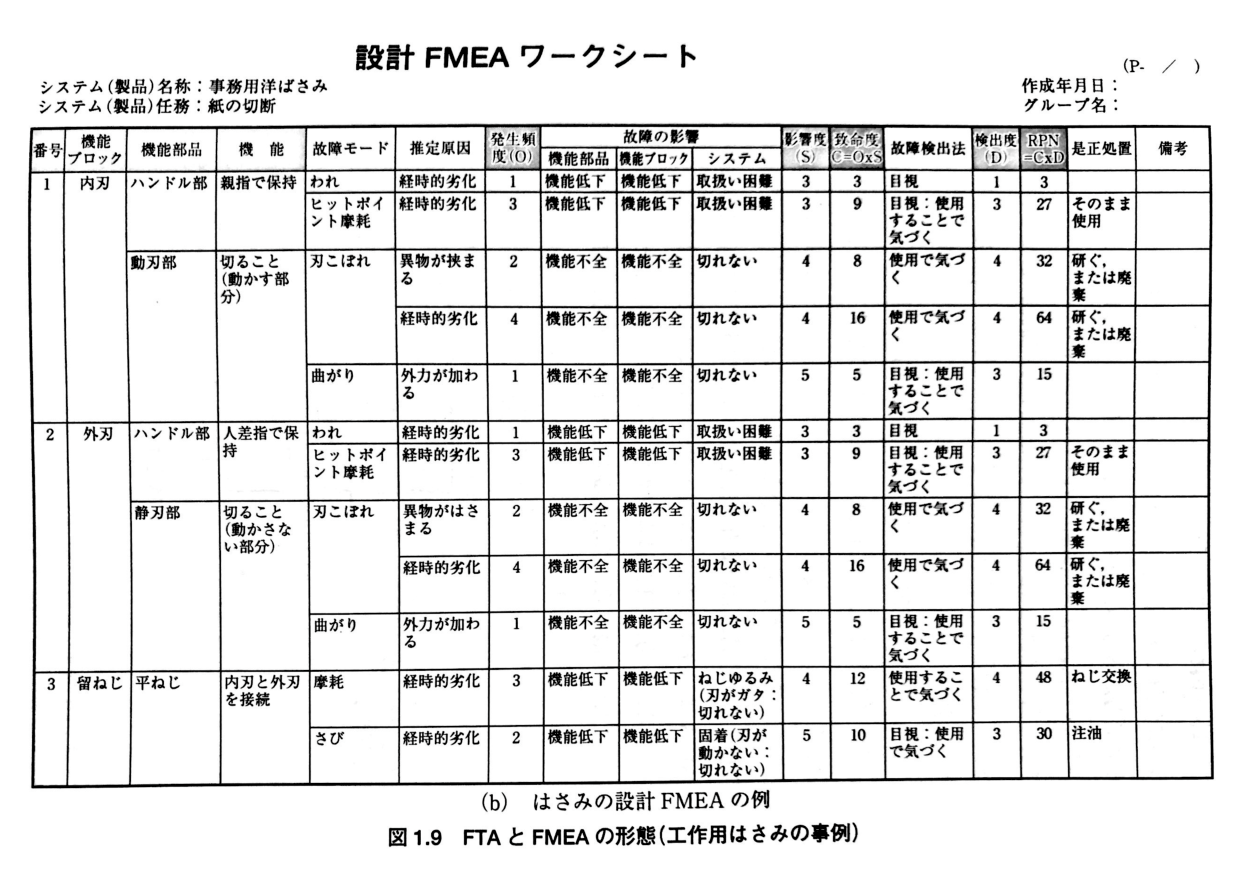
\includegraphics[width=15cm]{safety_assurance_contents/ch2images/192.eps}
\end{center}
\caption{FMEAの形態(工作用はさみの事例)}
\label{192}
\end{figure}
(c)は、はさみで紙が切れないという結果の事象を取り上げて、その原因を探るFTAの一部を示す。FTAは木構造の解析手法である。主な論理ゲートはANDゲート(論理積)とORゲート(論理和)である。

一般にシステムはサブシステムに、サブシステムはコンポーネントに、というように、順次、下位の構成要素に分解される。最終的にこれ以上分解できないレベルにいたる。システムとしては、階層的に分解できる構造であれば、ハードウエアでも、ソフトウエアでも、プロセスでも、あるいはそれらの複合でもよい。FMEAは下位の階層の悪さ加減が上位の階層の悪さ加減にどのように影響するかを表形式上で論理的に解析する手法である。FTAは逆に上位の階層の悪さ加減の原因となる下位の階層の悪さ加減を木構造で論理的に解析する手法である。FMEAは単一の原因が及ぼす複数の結果を網羅的に洗い出すのに優れた手法であるが、複数の原因によって及ぼされる結果の洗い出しは難しい。一方、FTAは複数の原因によって及ぼされる結果も表現できるが、網羅性が十分ではない。両者は相補的かつ相乗的に用いられている。
\section{FTA(Fault Tree Analysis、故障の木解析)}
FTAは、「なぜなぜ」を繰り返すことで、重大な故障やトラブルの発生要因を下方に向かって木構造として展開し、網羅した要因の中から重要な要因を抽出する。1979年にスリーマイル島で発生した原子力事故の解析の際、マサチューセッツ工科大学教授のRasmussenが原因の特定に使用したことでその有効性が評価され広まった手法である。
\subsection{FT図を読む}
FT図は、視覚的に故障に至るメカニズムが大変わかりやすく表現されている。FT図の記号は、イベントを示す事象記号と、それらの間の因果関係を示す論理記号とに分けられる。表\ref{43}にある4つの記号の意味を理解できれば、ほとんどのFT図を読むことができる。
\begin{table}[htbp]
\caption{FTAで用いる基本的な記号}
\begin{center}
%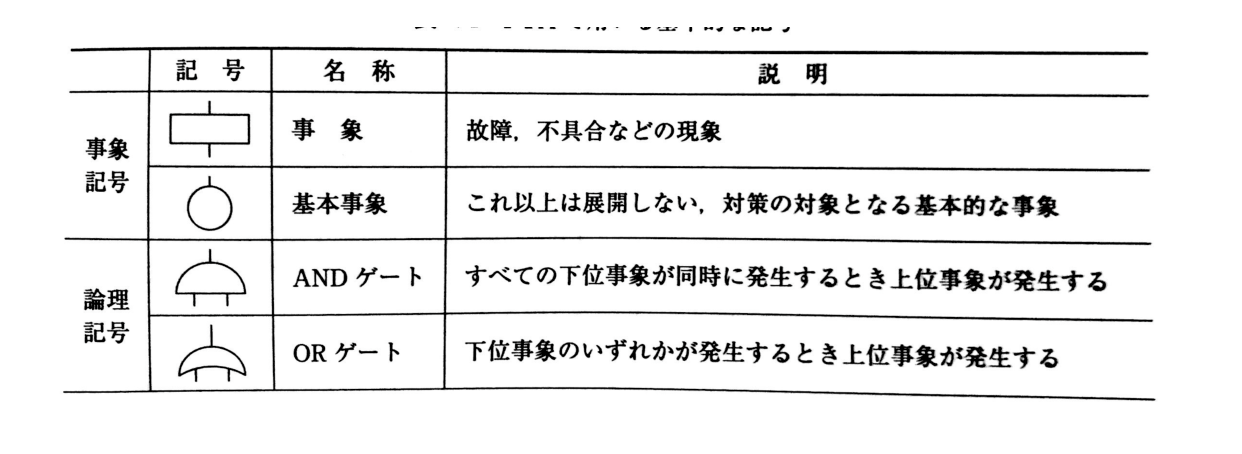
\includegraphics[width=13cm]{safety_assurance_contents/ch2images/44.eps}
\end{center}
\label{43}
\end{table}
さらに、表\ref{44}のノードも用いられる。
\begin{table}[htbp]
\caption{FTAで用いる便利な記号}
\begin{center}
%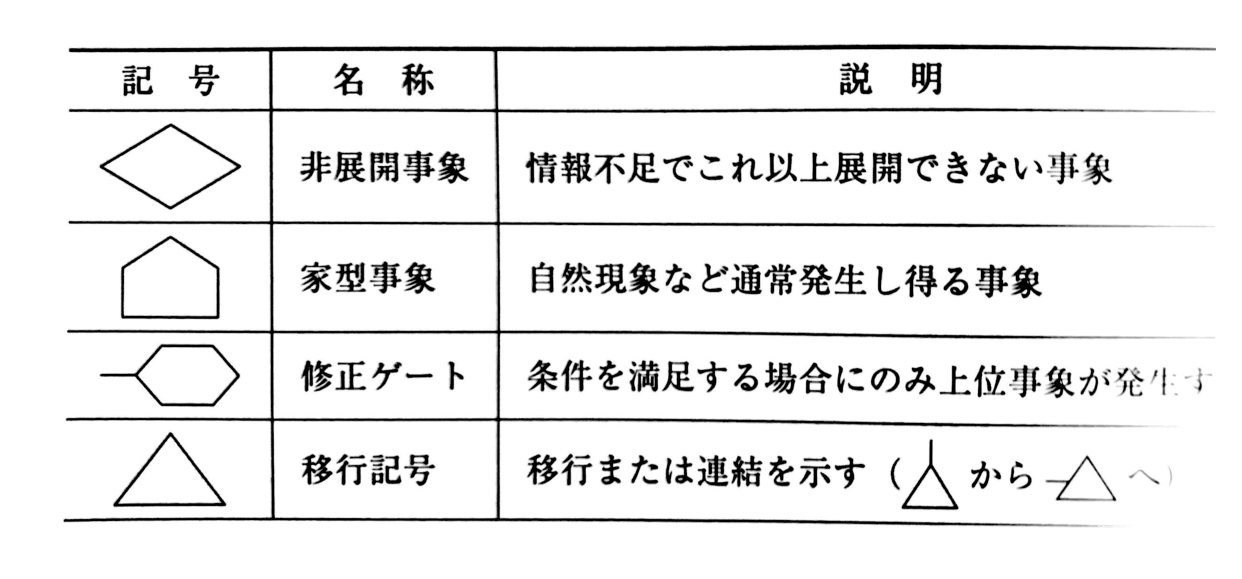
\includegraphics[width=11cm]{safety_assurance_contents/ch2images/45.eps}
\end{center}
\label{44}
\end{table}
FT図の例を図\ref{415}に示す。トップ事象である欠報の原因には「火災の検知信号が届かない」不具合と「ブザーが鳴らない」不具合とがあり、いずれか一方の原因で欠報に陥ることが示されている。さらに、その2つ以外に原因がないこと、あるいは他の原因は無視してよいことを示している点が重要である。この必要十分性は、熟練者でもしばしば見落とす点である。一方のANDゲートは、すべての下位事象が同時に発生するときに上位事象が発生することを示す記号で、並列型に対応する。「火災の検知信号が届かない」事象は、冗長に設置された2つのセンサ系A,Bが同時に故障しているときのみ発生する事象となる。
\begin{figure}[htbp]
\begin{center}
%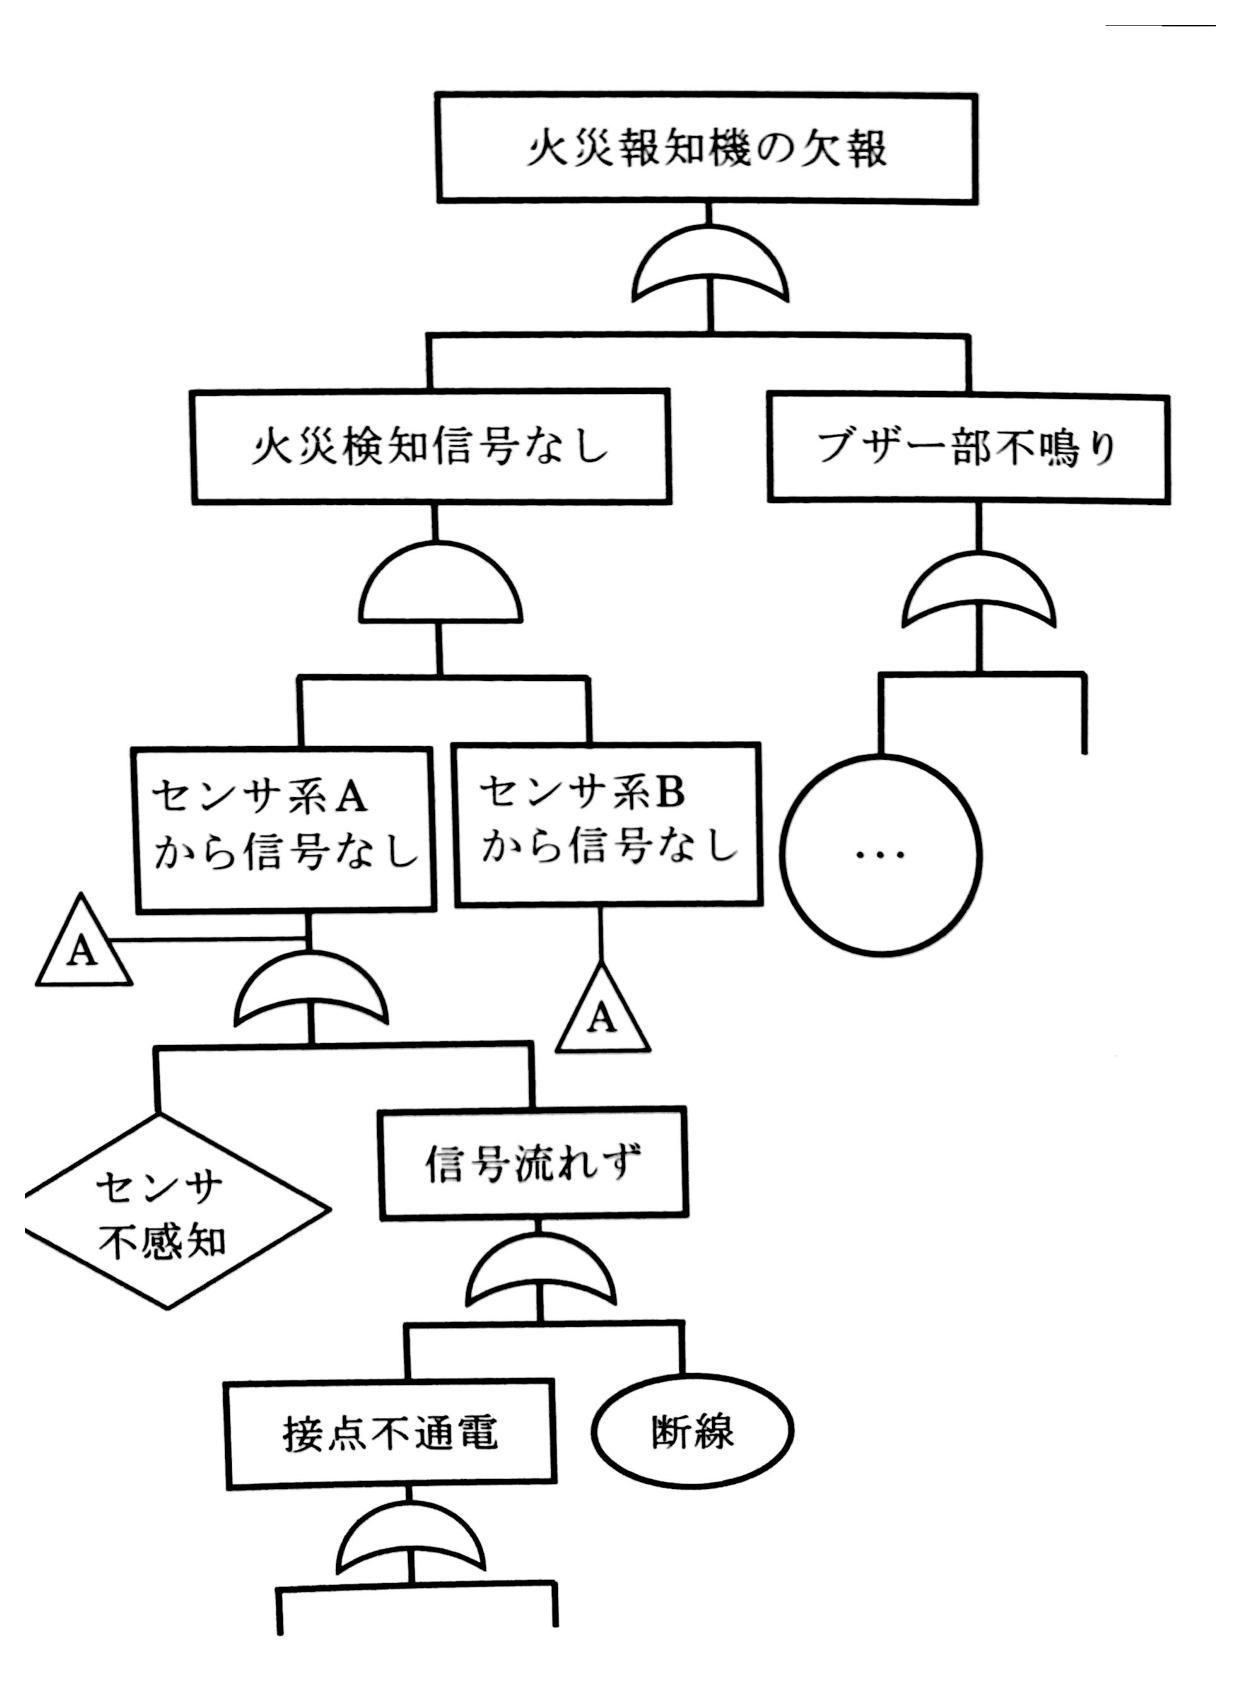
\includegraphics[width=7cm]{safety_assurance_contents/ch2images/145.eps}
\end{center}
\caption{FT図の例}
\label{415}
\end{figure}
FTAには、
\begin{itemize}
\item トップ事象と基本事象との因果関係が視覚的に示され、多様な事象間関係を把握しやすい。
\item ANDゲートにより多重故障を解析できる。
\end{itemize}
などの特徴がある。
\subsection{FT図の作成}
FTAの実施は、FT図の作成とFT図の解析の2つのステップで構成される。ここでは作成までの手順を説明する。
\begin{enumerate}
\item FTA実施の準備。対象製品を熟知する技術者と品質保証担当者を含めた3名から6名程度のメンバーで実施する。設計資料、図面、材料部品リストや想定使用状況、関連するトラブル、クレーム情報、特に不具合に関する情報を集める。
\item 解析対象の機能の理解。FTAで解析する対象製品の構造や機能について、参加者全員で十分理解する。自分の専門とする部分や分野に対象を限定することなく、周辺との関係なども理解することが重要である。
\item トップ事象の選定。信頼性や安全性を損なうような「発生することが望ましくない」トップ事象を注意深く選定する。その際、1. 明確に定義できる事象、2. 多くの下位事象の結果として発生する事象、3. 設計の中で技術的に対処できる基本事象が予想される事象、であることが望ましい。1が最も重要な要件であり、「明確」なとは、その事象発生の有無の判断が人によって異なることはない、との意味である。例えば「エアバッグが開かない(不動作故障)」、「エアバッグが不要のときに開く(誤作動故障)」などは、トップ事象としてふさわしい。しかし「***の満足度が低い」、「***の回転が不安定」などは、その範囲(基準値)が不明瞭であり適さない。また一見良さそうに見える「排気ガス規制の基準値を満たしていない」のような表現も避けるべきである。ガスの種類や基準値は時代と共に変化するので、「排気ガスCOの規制基準値**ppmを満たさない」などの具体的な基準値を明記する必要がある。2.は、FTA解析はマンパワーが必要となるので、できるだけ重要なトップ事象を扱う、という意味である。3.は、設計時に、FT図作成に関わる技術者が基本事象まで書ききることができるようにするためである。
\item トップ事象の1次要因への展開。トップ事象の1次要因を、製品の構造や機能、手順1で準備した情報などを基に列挙し、論理記号を用いて因果関係を明確に図示する。

展開する方法は大きく分けて2つある。
\begin{enumerate}
\item 構造(信頼性ブロック図)からの作成。あるシステムが信頼性ブロック図で構造が示される場合、直列系の部分をORゲートに、並列型部分をANDゲートに対応させることで、FT図を容易に作成できる。
\item 機能を考えて作成。実際には、信頼性ブロック図を基にFT図全てを作成できるケースは多くない。構成要素の機能に着目して、トップ事象の直接の原因である1次要因を抽出し、さらにそれらの原因である2次要因を抽出するという具合に、意味を考えてトップダウンに作成することになる。
\end{enumerate}
1次要因への展開は、最も頭を悩ませるステップだが、重要な箇所であり、時間をかけるべき手順である。システムを構成するサブシステムごとに空間的に分割し、それぞれを解析するとの方針がとられることが多いが、それよりも、エネルギーの流れに注目するなど、機能的な側面から1次要因を分解すると、装置間の相互作用などを見失うことが少なく、効果的な木になることが多い。
\item トップ事象の2次要因以下への展開。展開可能な1次要因に関して、さらになぜなぜ分析を続け、2次要因、3次要因を列挙、基本事象または非展開事象に至るまで論理記号を用いて展開する。
\end{enumerate}
例題 図\ref{41}に示されるような、2つのセンサが並列に設置された自動照明器で、「照明が点灯しない」をトップ事象とするFT図を作成せよ。
\begin{figure}[htbp]
\begin{center}
%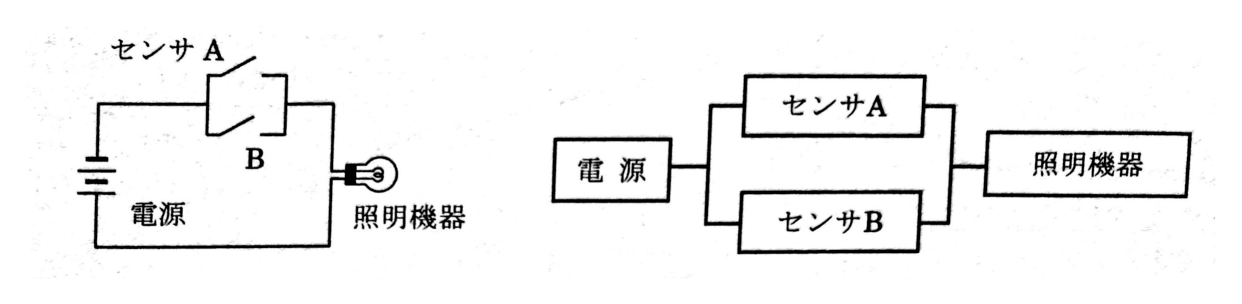
\includegraphics[width=10cm]{safety_assurance_contents/ch2images/41.eps}
\end{center}
\caption{照明設備の回路図と信頼性ブロック図}
\label{41}
\end{figure}

手順5まででFT図ができあがるが、効果的なFT図を作成するためのコツがある。
\renewcommand{\labelenumi}{\roman{enumi})}

\begin{enumerate}
\item 事象発生の有無が明確な表現にすること。トップ事象にかかわらず、中間事象や基本事象でも、事象発生の有無が人によりかわることのない、明確な表現にする。「**が弱い」、「**が不安定」などの表現はさけるべきである。
\item 基本事象では、事象を一意に特定できるように表現すること。基本事象レベルでの「接点故障」などの表現は不適切であり、それらの状況により対策が異なる。基本事象では、FT図の作成者に聞くことなく、その状況を一意に把握できる表現まで分解することが必要である。
\item 必要で十分な要因を漏れなく列挙しながらトップダウンで作成すること。各レベルでの要因抽出時に、思いつく要因の候補をあげればよい、という発想という発想では適切なFT図は得られない。特にORゲートの下位事象では、必要十分な要因を漏れなく列挙することが求められる。
\item 横のレベルをそろえながら分解すること。自分の得意な部分になると、いきなり詳細の部位の不具合要因がならぶことがよくある。1次、2次、とトップダウンで作成するが、それぞれのレベルに並ぶ事象の階層を合わせることが、見やすいFT図を作るコツである。
\end{enumerate}
\section{FT図で定量的に解析する}
FT図を作成すると、トップ事象を発生させる要因、およびその発生経路が明らかになる。それらを基に、解析のステップに移ることができる。

手順6では、トップ事象に対して改善効果が高いことが見込まれる基本事象を抽出するために、定量的評価法または定性的評価法を適用する。定量的評価法では、トップ事象の発生確率を求め、さらに、その確率を下げるためにはどの基本事象の発生確率を下げることが効果的かを特定する。そのためには、すべての基本事象の発生確率がわかっていることが前提となる。

手順7では、手順6で抽出された重要要因について、対策事項、対策方法を決定し、担当部署を決める。そして、対策実施後のフォローアップを確実に行う。

手順6におけえる定量的評価法では、トップ事象の発生確率を求め、さらにその確率を下げるためにはどの基本事象の発生確率を下げることが効果的かを特定する。そのためには、すべての基本事象の発生確率がわかっていることが前提となる。
\renewcommand{\labelenumi}{(\roman{enumi})}

\begin{enumerate}
\item トップ事象の発生確率。トップ事象の発生確率は、基本事象の発生確率から容易に推定することができる。論理記号に着目して、次の方法で上位事象の確率を算出していく。
\begin{enumerate}
\item ORゲート $\to$ 下位事象の発生確率の和
\item ANDゲート $\to$ 下位事象の発生確率の積
\end{enumerate}
例えば、図\ref{420}(b)で基本事象である各パソコンの故障の確率を0.001, プリンタの故障確率を0.0001とする。トップ事象の発生確率を推定する場合、パソコン故障の発生確率は、ANDゲートであるから、
\[Pr = 0.001 \times 0.001 = 1.0 \times 10 ^{-6}\]となり、トップ事象の発生確率は、ORゲートで結ばれているため、
\[Pr = 1.0 \times 10 ^{-6} + 1.0 \times 10^{-4} = 0.000101\]
となる。以下に注意したい。
\begin{itemize}
\item 事象の発生確率とは不信頼度$F$のことであり、故障率ではない。故障率は単位時間当たりの故障発生回数で定義されるので、ORゲートの場合は各構成要素の故障率の和で定義できるが、ANDゲートでは面倒な計算が必要となる。
\item ORゲートでの計算方法は近似式である。
\item ANDゲート、ORゲートでの計算の独立性が仮定されている。
\end{itemize}
\item 同一事象の排除。FT図においては、同一の基本事象、中間事象が2箇所に現れても構わない。ただし、定量的解析を行う場合、同一事象を一つにまとめたFT図に変形してから解析を進めなければ、誤った結果を導いてしまうことに注意すべきである。同一事象が複数含まれる場合には、事象間の独立性が失われるからである。図\ref{420}では、Treeとしては同値だが、トップ事象の発生確率を求める場合、同一の基本事象を一つにまとめた(b)図を用いなければならない。
\begin{figure}[htbp]
\begin{center}
%\includegraphics[width=13cm]{420.eps}
\end{center}
\caption{同じ意味の2つのFT図}
\label{420}
\end{figure}
より深刻な例として、2000年12月の京福電鉄の正面衝突事故がある。常用ブレーキも非常ブレーキも効かなかった事故であるが、通常、常用と非常用のブレーキは冗長化構造になっており、図\ref{421}の(a)のFT図が想定される。並列の2つのブレーキがあるにもかかわらず同時に故障に陥る確率は、1次要因がANDゲートで結ばれているため、積により小さな値になることが容易に想像できる。しかしこの車両のブレーキ装置では、常用と非常用で同一のブレーキレバーの角度の違いで操作する形式であり、ブレーキ制御部は同じものを使用していた。二重化されていたのは、圧縮空気の送風装置だけである。このため(b)のFT図でトップ事象の発生確率を算出する必要があった。
\begin{figure}[htbp]
\begin{center}
%\includegraphics[width=13cm]{421.eps}
\end{center}
\caption{常用ブレーキと非常ブレーキの多重故障の解析}
\label{421}
\end{figure}

\item トップ事象に大きな影響を与える基本事象の抽出。トップ事象の発生確率が推定されると、次に、どの基本事象の発生を抑えることがトップ事象の発生確率を下げるために効果的かを知ることができる。ORゲートの場合、トップ事象の発生確率は(重複事象がなく独立性が成立していれば)基本事象の発生確率のトータル和となるため、発生確率の最も高い基本事象から対策を講じれば良い。しかしANDゲートが含まれると容易ではない。
\end{enumerate}
\section{FT図で定性的に解析する}
多くの場合、基本事象の発生確率を推定することは難しい。基本事象の発生確率を前提とせず、トップ事象への影響の大きな基本事象を特定するための方法として、最小カット集合を利用した方法と構造重要度を利用した方法がある。
\subsection{最小カット集合を利用した方法}
最小カット集合とは、トップ事象を発生させ得る最小の基本事象の組み合わせである。例えば\ref{422}のTreeでは、$\{A,B\}, \{A,C\}$の2つが最小カット集合になる。この時、最小カット集合に共通の基本事象$A$が存在することから、$A$の発生を確実に抑えることができれば、トップ事象を回避することができる。すべての最小カット集合に共通の基本事象が存在するとは限らないが、一般には、できるだけ少ない基本事象の組み合わせで、すべての最小カット集合の発生を防止できるような組み合わせを探し出し対策を講じることで、トップ事象を防ぐことが可能となる。例えば最小カット集合が$\{A,B\},\{B,C,D\},\{B,E,F\},\{D,E,F,G\},\{G,H\}$ならば、$B$と$G$の2つの事象に確実な対策を施せばトップ事象を回避することができる。最小カット集合を得るためには、FT図のANDゲートを積、ORゲートを和で表し、ブール代数を用いて積で表した項の和(加法標準形)で全体を表現できれば、それら各項が最小カット集合である。ブール代数において、$0$は事象未発生、正常、$1$は事象発生、故障とする。図\ref{422}では
\[T=A\cdot (B+C) = A\cdot B + A \cdot C\]
となり、$\{A,B\}$, $\{A,C\}$の2つの最小カット集合が得られる。
\subsection{構造重要度を利用した方法}
構造重要度は、一つの基本事象に着目し、その事象が正規した時にトップ事象が発生する割合(他の事象の組み合わせ増加数)を表す。図\ref{422}の例で説明する。
\begin{figure}[htbp]
\begin{center}
%\includegraphics[width=13cm]{422.eps}
\end{center}
\caption{FT図とその基本事象とトップ事象}
\label{422}
\end{figure}
\renewcommand{\labelenumi}{(\roman{enumi})}

\begin{enumerate}
\item 最小カット集合を求める。$\{A,B\},\{A,C\}$が最小カット集合である。
\item 最小カット集合に基づき、基本事象とトップ事象との関係を表す真理表を作成する。
$A=B=1$(故障)、$A=C=1$のとき$T=1$とすればよい。
\item $A$に関する構造重要度$I_S(A)$を下記で求める。
\begin{itemize}
\item $X=$事象Aが故障時のトップ事象発生の組み合わせ数、
\item $Y=$事象Aが正常時のトップ事象発生の組み合わせ数としたとき、
\end{itemize}
\[I_S(A) = \frac{X-Y}{2^{n-1}},\]
すなわち$I_S(A)=\frac{3-0}{4}=\frac{3}{4}$となる。また$I_S(B)=I_S(C)=\frac{2-1}{4}=\frac{1}{4}$となり、Aの構造重要度はB,Cのそれよりも3倍となる。よって$A$を重点的に対策を取れば良いといえる。すべての基本事象の構造重要度を算出することで、トップ事象の回避への寄与度を知ることができるが、この値の算出は意外と面倒である。FTA解析用のソフトウエアでは自動的に計算され便利である。
\end{enumerate}
\section{FTA実施上の留意点}
FTAを実施する際に注意すべき点は下記の通りである。
\begin{enumerate}
\item 全ての基本事象の発生確率が必要であること。
\item 創発故障への対応。部品間の相互作用による創発故障を見落とさないためには、1次の分解で、構造ではなく、機能に着目して分解することに注意するとよい。
\item 動的変化への対応。FTAは基本的に静的な解析であり、動的変化を解析しにくい。トップ事象の発生確率も動的に変化するため、一定期間後のある時点での値で評価することに限定される。
\item 事後解析での活用。未然防止での利用を念頭に説明してきたが、故障解析や事故解析などの事後解析では確率値を利用した解析は行わない。実際に発生している真の原因を、多数の可能性がある要因の中から絞るためにFT図を利用するものであり、最小カット集合の中から、新の発生要因を絞り込むことが可能になる。
\end{enumerate}



\section*{参考文献}
本資料は「システムの信頼性と安全性、田中健次、朝倉書店」、「新FMEA技法、益田昭彦、高橋正弘、本田陽広、日科技連」を基にしている。
